\documentclass[12pt]{book}
\usepackage[a4paper,width=150mm,top=25mm,bottom=25mm]{geometry}         
\usepackage{amsmath}        
\usepackage{graphicx}        
\usepackage{xcolor}
\usepackage{float}
\usepackage{titlesec}
\usepackage[italian]{babel}
\usepackage{listings}
%\usepackage{enumitem}
%\setlist{nosep}

    
\definecolor{lightgray}{gray}{0.95}    
    
% Stile dei titoli dei capitoli    
\definecolor{gray75}{gray}{0.75}    
\newcommand{\hsp}{\hspace{20pt}}    
\titleformat{\chapter}[hang]    
{\Huge\bfseries}    
{\thechapter\hsp\textcolor{gray75}{|}\hsp}    
{0pt}    
{\Huge\bfseries}    

\begin{document}

"..."
\chapter{xen}
VMM nato come opensoruce paravirtualizzato.
\begin{figure}[H]
	\caption{Architettura xen}
	\centering
	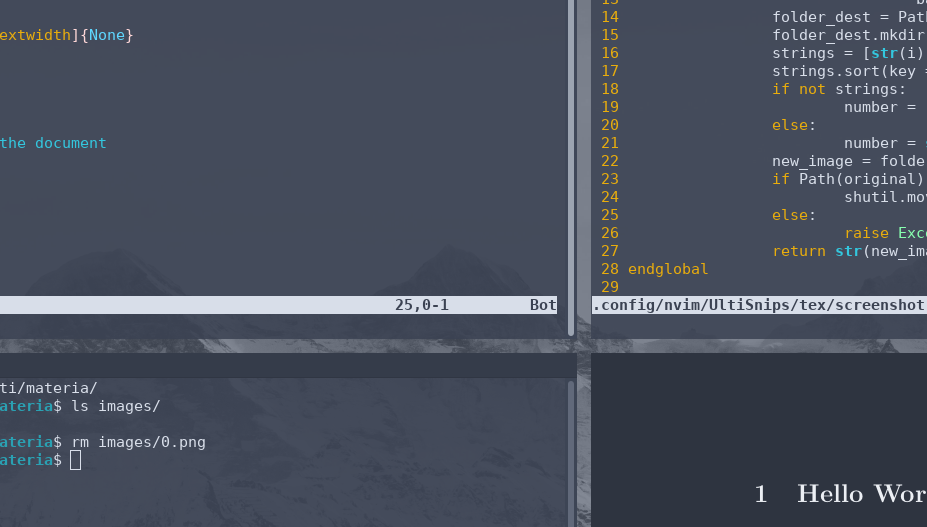
\includegraphics[width=0.8\textwidth]{/home/riccardoob/appunti/sistemi_operativi/images/0.png}
\end{figure}
Xen è un VMM di sistema, ovvero si appoggia direttamente sull'hardware e quindi può eseguire direttamente chiamate system call che necessita del rin 0.

Il vmm si occupa della virtualizzazione della CPU, della memoria e dei dispositivi per ogni macchina virtuale, qui definiti domain.

Xen offre una interfaccia di controllo in grado di gestire la divisione delle risorse tra i vari domini.
L'accesso a questa interfaccia è consentito soltanto da una speciale VM, la domain 0.

\section{Caratteristiche}
Data la natura \textbf{paravirtualizzata} delle VM gestite da xen, le VM possono eseguire direttamente system calls che vengono delegate al VMM tramite hypercalls.

Per quanto riguarda la \textbf{protezione}, i guest OS sono collocati nel ring 1.

\begin{figure}[H]
	\caption{Protezione e hypercalls guest OS}
	\centering
	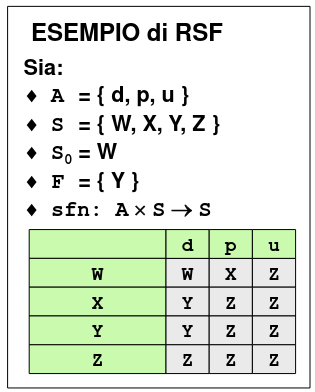
\includegraphics[width=0.85\textwidth]{/home/riccardoob/appunti/sistemi_operativi/images/1.png}
\end{figure}

\section{Gestione memoria e paginazione}

\subsubsection{Gestione della memoria}
Gli OS guest gestioscono la memoria virtuale mediante i meccanismi e le politiche tradizionali.

La soluzione adottata si basa sulle tabelle delle pagine delle VM:\\
Vengono mappate nella memoria fisica dal VMM (\textbf{shadow page tables}, possono essere accedute in scrittura soltanto dal VMM stesso ma sono disponibili in modalità read-only ai guest.

In caso di necessità di update, il VMM valuta la richiesta e la esegue.

Per alleggerire l'onere del procedimento di update, viene implementato il \textbf{memory split}, per permettere una maggiore efficienza delle hypercalls: xen risiede nei primi 64MB del virtual address space.

\begin{figure}[H]
	\caption{Struttura virtual address space- memory split}
	\centering
	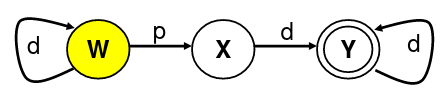
\includegraphics[width=0.6\textwidth]{/home/riccardoob/appunti/sistemi_operativi/images/2.png}
\end{figure}

I guest OS si occupano della paginazione, delegando al VMM la scrittura delle page table entries, una volta create sono disponibili in read-only per il guest che le ha richieste.

\begin{figure}[H]
	\caption{Creazione pagine dal VMM}
	\centering
	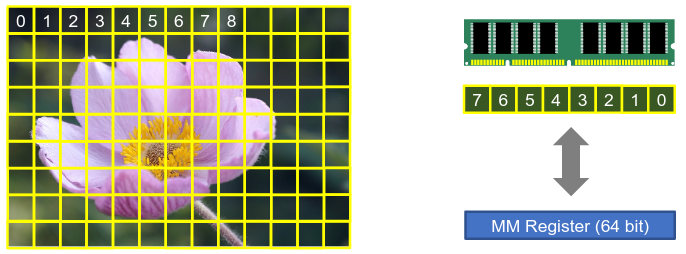
\includegraphics[width=0.7\textwidth]{/home/riccardoob/appunti/sistemi_operativi/images/3.png}
\end{figure}

\subsubsection{Creazione di un processo}

Il SO richiede una nuova tabella delle pagine al VMM:\\
\begin{itemize}
	\item aggiunte alla tabella le pagine appartenenti al segmento di xen
	\item xen registra la nuova tabella e acquisisce il diritto di scrittura esclusiva
	\item ogni successiva update da parte del guest provoca un protection-fault, comporta la verifica e l'aggiornamento della PT
\end{itemize}

\begin{figure}[H]
	\caption{Creazione di un processo}
	\centering
	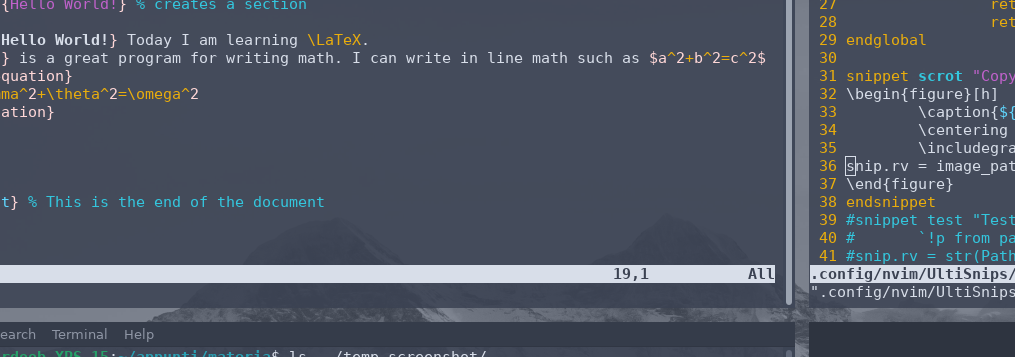
\includegraphics[width=0.85\textwidth]{/home/riccardoob/appunti/sistemi_operativi/images/4.png}
\end{figure}

\subsubsection{Balloon process}
Dato che la paginazione è a carico dei guest, il VMM necessita di avere un meccanismo per reclamare da altre macchine virtuali pagine di memoria meno utilizzate.
Su ogni macchina virtuale è in esecuzione un \textbf{ballon process} che, in caso di necessità, si "gonfia" per ottenere altre pagine che poi cede al VMM.

\section{Virtualizzazione della CPU}
Il VMM definisce una archiettura simile a quella del processore, con istruzioni privilegiate sostituite da opportune hypercalls.

Il VMM si occupa dello scheduling delle macchine virtuali: \textbf{Borrowed Virtual Time} scheduling algorithm:
\begin{itemize}
	\item si basa sulla nozione di virtual-time
	\item algoritmo general-purpose, consente di ottenre schedulazioni efficienti in caso di vincoli stringenti
\end{itemize}

Esistono due clock:
\begin{itemize}
	\item real-time, inizia al boot
	\item virtual-time, associato a VM, avanza solo quando la VM esegue
\end{itemize}

\begin{figure}[H]
	\caption{Virtualizzazione dell'I/O}
	\centering
	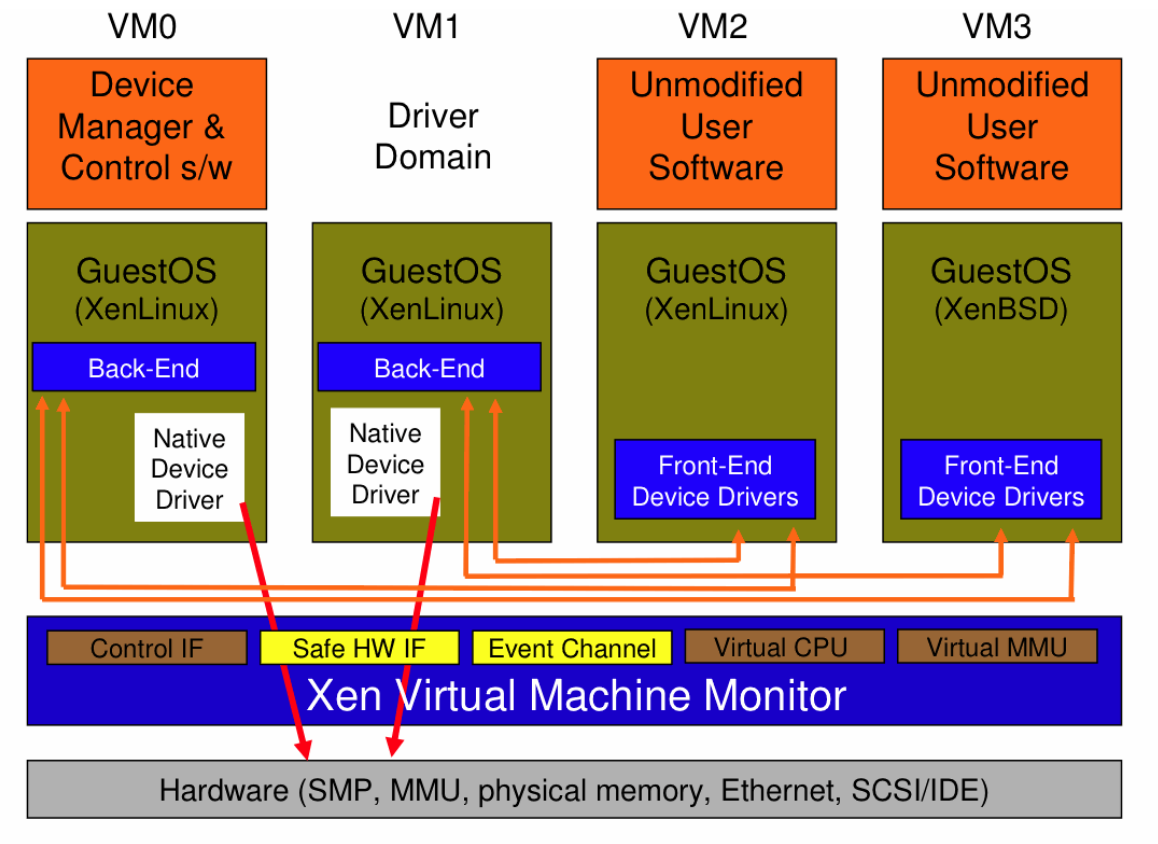
\includegraphics[width=0.7\textwidth]{/home/riccardoob/appunti/sistemi_operativi/images/5.png}
\end{figure}

Esiste un \textbf{back-end driver} per ogni dispositivo, il suo driver è isolato all'interno di una particolare macchine virtuale (tipicamente dom0), ha accesso diretto all'hardware.

Ogni guest prevede un \textbf{front-end driver} virtuale semplificato che consente l'accesso al device tramite il back-end.

Questa tecnica comporta una semplificazione della portabilità a scapito della necessità di comunicaazione don il back-end attraverso degli asynchronous I/O rings.
\begin{figure}[H]
	\caption{I/O rings}
	\centering
	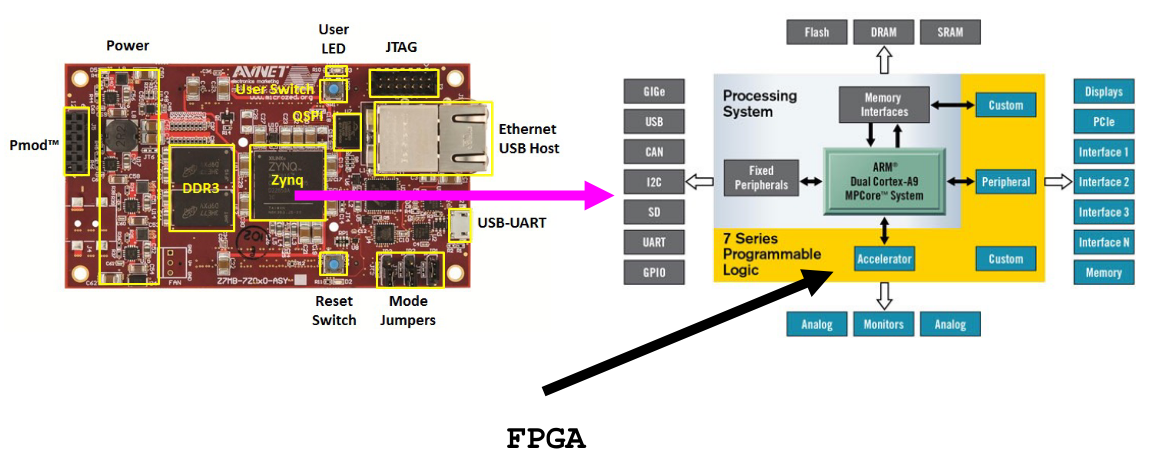
\includegraphics[width=0.75\textwidth]{/home/riccardoob/appunti/sistemi_operativi/images/6.png}
\end{figure}

\section{Gestione interruzioni e eccezioni}
La gestione delle interruzione viene virtualizzata in modo da lasciare a ogni guest la gestione delle interruzioni, il vettore punta direttamente alle routine del kernel guest.

Il page-fault è un caso particolare, nel quale è necessario l'intervento del VMM, in quanto l'indirizzo che ha provocato il page-fault è contenuto nel registro CR2, inaccessibile al guest: il guest punta a codice xen che esegue una copia del CR2 all'interno di una variabile nello spazio guest.

\section{Live migration in xen}
La migrazione è \textbf{guest-based}: il comando di migrazione viene eseguite da un demone di migrazione nel domain0 del server di origine della macchine da migrare.

La realizzazione si basa sulla modalità pre-copy, le pagine da migrare vengono compresse per ridurre l'occupazione di banda.

\begin{figure}[H]
	\caption{Migrazione live}
	\centering
	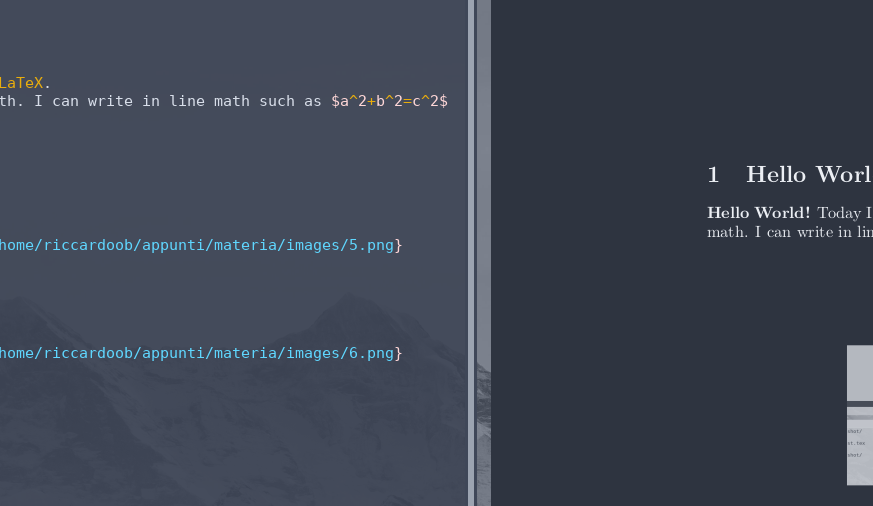
\includegraphics[width=0.8\textwidth]{/home/riccardoob/appunti/sistemi_operativi/images/7.png}
\end{figure}


\chapter{Protezione}
    
\subsubsection{Sicurezza}
Insieme delle tecniche per regolamentare l'accesso degli utenti al sistema di elaborazione. La sicurezza impedisce accessi non autorizzati al sistema e i conseguenti tentativi dolosi di alterazione e distruzione dei dati.

Meccanismi per \textbf{identificazione}, \textbf{autenticazione} e \textbf{autorizzazione} di utenti "fidati".
    	
\subsubsection{Protezione}
Insieme di attività volte a garantire il controllo dell'acecsso alle risorse logiche e fisiche da parte degli utenti autorizzati all'uso di un sistema di calcolo.

Definizione, per ogni utente autorizzato, di:
\begin{itemize}
	\item quali \textbf{risorse} sono accessibili
	\item quali \textbf{operazioni} può effettuare
\end{itemize}

Sono stabilite tramite tecniche di controllo degli accessi.

\section{Protezione}
In un sistema, il controllo degli accessi si esprime tramite la definizione di tre livelli concettuali:
\begin{itemize}
	\item modelli
	\item politiche
	\item meccanismi
\end{itemize}

\subsection{Modelli}
Un modello di protezione definisce \textbf{soggetti}, \textbf{oggetti} ai quali i soggetti possono accedere e i \textbf{diritti} di accesso:
\begin{itemize}
	\item oggetti, risorse fisiche e logiche alle quali applicare limitazione di accesso;
	\item soggetti, entità che possono richiedere l'accesso agli oggetti, utenti e processi;
	\item diritti di accesso, operazioni con le quali è possibile operare sugli oggetti;
\end{itemize}

\subsubsection{Dominio di protezione}
Ad ogni soggetto è associato un \textbf{dominio} che rappresenta l'ambiente di protezione nel quale il soggetto esegue, il dominio specifica i diritti di accesso posseduti dal soggetto nei confronti di ogni risorsa.

Un dominio di protezione è \textbf{unico per ogni soggetto}, mentre un processo può eventualmente cambiare dominio durante la sua esecuzione.

\subsection{Politiche}
Le \textbf{politiche di protezione} definiscono le regole con le quali i soggetti possono accedere agli oggetti.

Classificazione delle politiche:
\begin{itemize}
	\item \textbf{Discetional Access Control} (DAC): il creatore di un oggetto controlla i diritti di accesso per quell'oggett (UNIX), definzione delle politiche decentralizzata.
	\item \textbf{Mandatory Access Control} (MAC): i diritti di accesso vengono definiti in modo centralizzato. Installazione ad alta sicurezza (es. enti gonvernativi)
	\item \textbf{Role Based Access Control} (RABC): un ruolo ha specifici diritti di accesso alle risorse, gli utenti possono appartenere a diversi ruoli, i diritti sono assegnati in modo centralizzato.
\end{itemize}

\subsubsection{Principio del privilegio minimo}
Ad ogni soggetto sono garantiti i diritti di accesso solo agli oggetti strettamente necessari per la sua esecuzione, è una caratteristica desiderabile in tutte le politiche di protezione.

\subsection{Meccanismi}
I meccanismi di protezione sono gli strumenti messi a disposizione dal sistema di protezione per imporre una determinata politica.

\subsubsection{Principi di realizzazione}

\begin{itemize}
	\item \textbf{Flessibilità} del sistema di protezione, i meccanismi di protezione devono essere sufficientemente generali per consentire l'applicazione di diverse politiche;
	\item \textbf{Separazione} tra meccanismi e politiche, la politica definisce il \textit{cosa} va fatto e il meccanismo il \textit{come} va fatto.
\end{itemize}

In UNIX si utilizza la politica DAC e il SO offre un meccanismo per definire e interpretare i tre bit dei permessi.

\subsection{Dominio di protezione}
Un dominio definisce una serie di coppie che associano un oggetto all'insieme delle operazioni che il soggetto associato al dominio può eseguire.

Ogni dominio è associato univocamente a un soggetto.

\subsubsection{Domini disgiunti o con diritti di accesso comune}

Esiste la possibilità per due o più soggetti di effettuare alcune opezione comuni su un oggetto condiviso, le operazioni vengono svolte da processi che operano per conto di soggetti, tuttavia un processo appartiene a un solo dominio in ogni istante.

\subsubsection{Associazione tra processo e dominio}

\paragraph{Modalità statica}
L'insieme di risore disponibili a un processo rimane \textbf{statico} durante tutto il suo tempo di vita.

L'associazione statica non è adatta nel caso si voglia limitare per un processo l'uso delle risorse a quello strettamento necessario.

\paragraph{Modalità dinamica}
L'associazione tra processo e dominio varia durante l'esecuzione del processo.

\subsubsection{Matrice degli accessi}

Un sistema di protezione può essere rappresentato a livello astratto utilizzando una \textbf{matrice degli accessi}.

\begin{figure}[H]
	\caption{Matrice degli accessi}
	\centering
	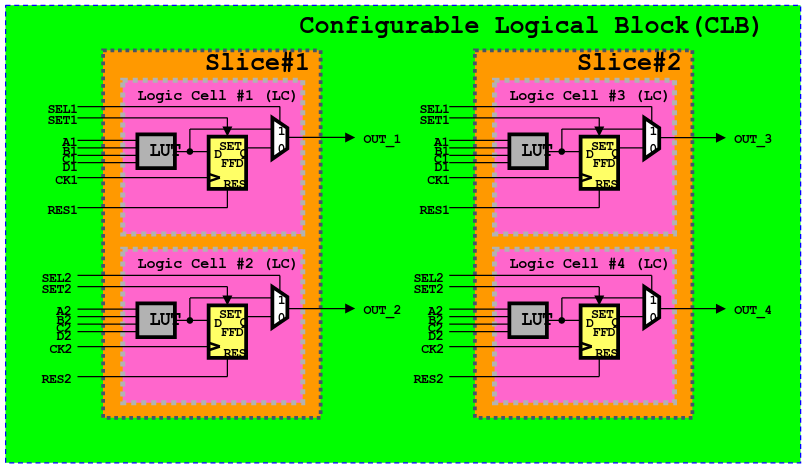
\includegraphics[width=0.8\textwidth]{/home/riccardoob/appunti/sistemi_operativi/images/8.png}
\end{figure}
\begin{itemize}
	\item Ogni riga è associata a un oggetto
	\item Ogni colonna è associata a un oggetto
\end{itemize}

La matrice consente di rappresentare il modello e le politiche valide nel sistema considerato, specificando
\begin{itemize}
    \item \textbf{soggetti}
    \item \textbf{oggetti}
    \item \textbf{diritti} accordati ai soggeti sugli oggetti
\end{itemize}

Le informazioni contenute nella matrice possono variare nel tempo, per effetto di operazioni che ne consentono la modifica $\rightarrow$ le informazioni contenute nella matrice all'istante t rappresenta lo \textbf{stato di protezione} del sistema in t.

La matrice degli accessi offre ai \textbf{meccanismi} di protezione le informazioni che consentono di verificare il rispetto dei vincoli di accesso.

Il meccanismo di protezione:
\begin{itemize}
    \item verifica se ogni richiesta di accesso che proviene da un processo che opera in un determinato dominio è consentita oppure no
    \item autorizza l'esecuzione delle richieste se permesse
    \item esegue la modifica dello stato di protezione in seguite ad ogni richiesta autorizzata da pate di un processo
\end{itemize}

Quando un operazione $M$ deve essere eseguita nel dominio $D_i$ sull'oggetto $O_j$, il meccanismo consente di controllare che $M$ sia contenuta nella casella \texttt{access(i,j)}.  

\subsection{Modello di Graham-Denning}
La modifica controllata dello stato di protezione può essere ottenuta tramite un opportuno insieme di comandi (Graham e Denning, 1972):
\begin{itemize}
    \item create object
    \item delete object
    \item create subject
    \item delete subject
    \item read access right
    \item grant access right
    \item delete access right
    \item transfer access right
\end{itemize}

\subsubsection{Propagazione dei diritti di accesso}
La possibilità di copiare un diritto di accesso per un oggetto da un dominio ad un altro della matrice di accesso è indicato con il \underline{copy flag \texttt{*}}.

Un soggetto $S_i$ può trasferire un diritto di accesso $\alpha$ per un ogget $X$ ad un altro soggetto $S_j$ ad un altro soggetto $S_j$ solo se $S_i$ ha accesso a $X$ con il diritto $\alpha$, e $\alpha$ ha il copy flag.

L'operazione di propagazione può essere realizzata in due modi:
\begin{itemize}
    \item trasferimento del diritto, viene perso dal soggetto originale
    \item copia del diritto: viene mantenuto dal soggetto originale
\end{itemize}

\subsubsection{Diritto owner}
Se un soggetto $S_i$ ha il diritto \textbf{owner} su un oggetto $X$, può assegnare/revocare un qualunque diritto di accesso a un soggetto $S_j$.

\subsubsection{Diritto control}
Se un soggetto $S_i$ ha il diritto \textbf{control} su un soggetto $S_j$, può assegnare/revocare un qualunque diritto di accesso a un soggetto $S_j$ per un qualsiasi oggett $X$.
\begin{figure}[H]
    \caption{Matrice degli accessi}
    \centering
    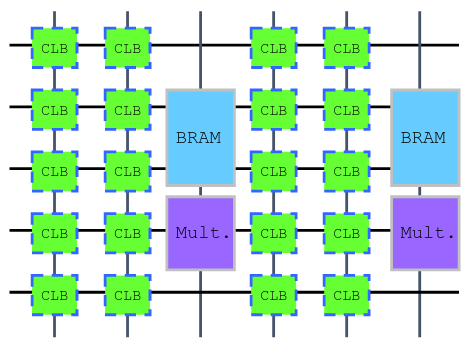
\includegraphics[width=0.6\textwidth]{/home/riccardoob/appunti/sistemi_operativi/images/9.png}
\end{figure}

\subsubsection{Switch}
Un processo che esegue nel dominio del soggetto può commutare al dominio di un altro soggetto $S_j$. L'operazione è consentita solo se il diritto \textbf{switch} appartiene a \texttt{access($S_i$,$S_j$)}.

\subsection{Realizzazione della matrice degli accessi}
La matrice degli accessi è una notazione astratta, realizzare in memoria una struttura dati matriciale $N_s \times N_o$ non sarebbe ottimale, considerando il fatto che è una matrice sparsa.

Esistono due approcci possibili:
\begin{itemize}
    \item \textbf{Access Control List} (ACL): rappresentazione per colonne, ogni oggetto possiede una lista che contiene tutti i soggetti che possono accedervi, con relativi diritti di accesso.
    \item \textbf{Capability List}: Rappresentazione per righe, ogni soggetto possiede una lista che contiene gli oggetti accessibili, con relativi diritti di accesso.
\end{itemize}

\subsubsection{Access control list}
La lista degli accessi, per ogni oggetto, è rappresentata da un insieme di coppie:

{\centering
\texttt{<soggetto, insieme dei diritti>} \par}   

limitatamente ai soggetti con un insieme non vuoto di diritti per l'oggetto.

Quando si deve eseguire l'operazione $M$ su un oggetto $O_j$ da parte di $S_i$, si cerca nella lista degli accessi 

{\centering
\texttt{<$S_i$,$R_k$>}, con $M$ appartente a $R_k$\par}   

La ricerca può essere fatta in precedenza su una lista di default che contiene i diritti di accesso applicabili a tutti gli oggetti.

\paragraph{Utenti e gruppi} Solitamente ogni soggetto rappresenta un singolo utente, molti sistemi tuttavia hanno il concetto di \textbf{gruppo di utenti}, liste di utenti identificate da un nome ch e possono essere inclusi nell'ACL.

Se i gruppi sono presenti, l'ACL ha la seguente forma:

{\centering
$UID_1$ $GID_1$: \texttt{<insieme di diritti>} \par}   

con UID \underline{user identifier} e GID \underline{group identifier}.

\subsubsection{Capability list}
La lista delle capability, per ogni soggetto, è la lista di elementi ognuno dei quali:
\begin{itemize}
    \item è associato a un oggetto a cui il soggetto può accedere
    \item contiene i diritti di accessi consentiti su tale oggetto
\end{itemize}
ogni elemento della lista prende il nome di \textbf{capability} .

La capability si compone di un identificatore (indirizzo) che identifica l'oggetto e la rappresentazione dei vari diritti concessi.

Quando $S$ intende eseguire una operazione $M$ su $O_j$, il meccanismo di protezione controlla se tra le capability di $S$ ne esista una relativa ad $O_j$ che contiene $M$

Le liste di capability devono essere protette da manomissioni, proprietà ottenibile spostando l'effettiva lista nello spazio del kernerl e esponendo soltato un riferimento a tale lista.

L'utilizzo di una sola delle due soluzioni è inefficiente, in ACL tutti i diritti di un soggetto sono sparsi nelle varie ACL degli oggetti, e nelle CL tutti i diritti di accesso applicabili a un oggeto sono sparsi nelle varie CL dei soggetti.

\subsubsection{Revoca dai diritti di accesso}

In un sistema di protezione dinamica può essere necessario revocare i diritti di accesso per un oggetto, la revoca può essere:
\begin{itemize}
    \item \textbf{generale} o \textbf{selettiva}: valere per tutti gli utenti o solo per un sottoinsieme
    \item \textbf{parziale} o \textbf{totale}: tutti i diritti o un sottoinsieme
    \item \textbf{temporanea} o \textbf{permanente}: il diritto di accesso non sarà più disponibile, oppure potrà essere successivmente riottenuto
\end{itemize}

In ACL revocare diritti su un oggetto risulta semplice, in quanto sono raccolte in un unica entri della lista, al contrario di CL nel quale è necessario agire su ogni entry che riguarda anche l'oggetto in esame.

\subsubsection{Cancellazione/aggiunta di un utente}
In un sistema di multi-user è possibile modificare l'insieme degli utenti autorizzati:
\begin{itemize}
    \item \textbf{cancellazione} utente esistente $\rightarrow$ eliminazione di ogni traccia dell'utente dal sistema di protezione
    \item \textbf{aggiunta} nuovo utente $\rightarrow$ inizializzare il sistema di protezione per l'utente e il suo accesso alle risorse
\end{itemize}

In ACL eliminare un utente è complesso, in quanto è necessario agire su ogni entry che riguarda anche l'utente in esame, al contrario di CL nel quale basta eliminare l'entry associata all'utente.

Si implementa spesso una soluzione mista, con ACL (unita a una cache in RAM per accessi frequenti), tutte le operazioni successiva su una risorsa vengono effettuate tramite il fd e le capability.

\section{Sicurezza}

La sicurezza riguarda il controllo degli accessi al sistema, la protezione di un sistema può essere inefficace se un utente non fidato riesce a fare eseguire programmi che agiscono sulle risorse del sistema.

\subsection{Sicurezza multilivello}

La maggior parte dei sistemi operativi permette ai singoli utenti di gestire accesso ai loro file e oggetti, tuttavia in alcuni ambiti è richiesto un più stretto controllo sulle regole di accesso alle risorse, ottenibile stabilendo regole più generali (MAC).

L'organizzazione che gestisce il sistema definisce le politiche MAC che stabiliscono \underline{regole generali} su chi può accedere e a che cosa tramite l'adozione di un \textbf{modello di sicurezza}.

I modelli di sicurezza più usati sono:
\begin{itemize}
    \item modello \textbf{Bell-La Padula} 
    \item modello \textbf{Biba} 
\end{itemize}

Entrambi sono modelli multilivello.

\subsection{Modelli di sicurezza multilivello}
I \textbf{soggetti} (utenti) e gli \textbf{oggetti} (risorse) sono classificati in \textbf{livelli} di accesso:
\begin{itemize}
    \item \underline{clearance levels} 
    \item \underline{sensititivity levels} 
\end{itemize}

Il modello fissa inoltre le \textbf{regole di sicurezza} che controllano il flusso delle informazioni tra i livelli.

\subsection{Modello Bell-La Padula}
Progettato principalmente per organizzazioni militari che necessitano di \textbf{confidenzialità}  delle informazioni. Associa a un sistema di protezione due regole di sicurezza MAC che stabiliscono il flusso di propagazione delle informazioni nel sistema.

Livelli di sensibilità degli oggetti:
\begin{itemize}
    \item non classificato
    \item confidenziale
    \item segreto
    \item top secret
\end{itemize}

Livelli di autorizzazione (clearance) per i soggetti, assegnati a seconda del ruolo dell'utente nell'organizzazione ovvero dei documenti a quali è consentito accedere.

\subsubsection{Regole di sicurezza}
\begin{itemize}
    \item \underline{proprietà di semplice sicurezza}: un processo in esecuzione al livello di sicurezza k può leggere solo oggetti al suo livello o a livelli inferiori
    \item \underline{proprietà \texttt{*}} : un processo in esecuzione allivello di sicurezza k può scrivere solamente oggetti al suol livello o a quelli superiori
\end{itemize}

Questo significa che i processi possono leggere verso il basso e scrivere verso l'alto, ma non il contrario, quindi il \underline{flusso delle informazioni} è dal basso verso l'alto.

\begin{figure}[H]
    \caption{Diagramma sicurezza Bell-La Padula}
    \centering
    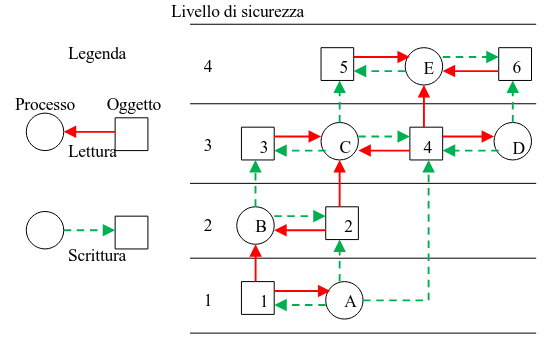
\includegraphics[width=0.8\textwidth]{/home/riccardoob/appunti/sistemi_operativi/images/14.png}
\end{figure}

Questo modello non è concepito per mantenere l'integrità dei dati ma per conservare segreti, è infatti ammesso sovrascrivere informazioni appartenenti a livelli superiori.

\subsubsection{Esempio - difesa cavalli di troia}

Si immagini un utente, Paolo, creatore del file \texttt{Fp} contenente una stringa riservata con permessi \texttt{r/w} solo per processi che appartengono a lui. Un utente ostile, Marco, ottenuto accesso al sistema, installa il file eseguibile \texttt{CT} e copia nel file system un file privato \texttt{Fm} che verrà utilizzato come "tasca posteriore".

Marco induce Paolo a eseguire il processo \texttt{CT}, che copia il contenuto di \texttt{Fp} in \texttt{Fm}, senza violare classiche regole di protezione (es. ACL).

Il modello, per prevenire attacchi di questo tipo, implementa 2 livelli di sicurezza, \textbf{privato} e \textbf{pubblico}:
\begin{itemize}
    \item ai processi e file di Paolo viene assegnato il livello \textit{riservato}
    \item ai processi e file di Marco viene assegnato il livello \textit{pubblico}
\end{itemize}

Quando il processo, avviato da Paolo con livello riservato, tenta di scrivere su \texttt{Fm} (pubblico) la proprietà \texttt{*} è violata e il tentativo è negato, nonostante ACL lo consenta.

La politica di sicurezza ha la precedenza sulle regole ACL.

\begin{figure}[H]
    \caption{Diagramma blocco cavallo di troia}
    \centering
    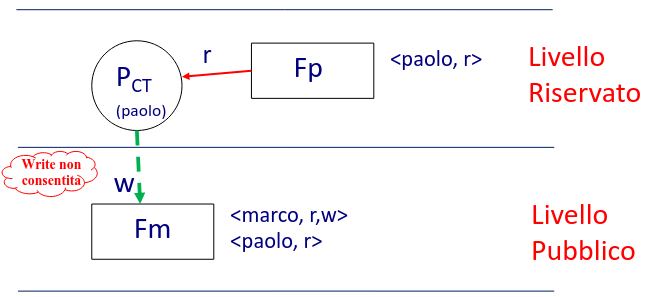
\includegraphics[width=0.8\textwidth]{/home/riccardoob/appunti/sistemi_operativi/images/15.png}
\end{figure}

\subsection{Modello Biba}

L'obiettivo di questo modello è l'integrità dei dati, diversamente dal Bell-La Padula.

\begin{itemize}
    \item \underline{proprietà di semplice sicurezza}: un processo in esecuzione al livello di sicurezza k può scrivere solo oggetti al suo livello o a livelli inferiori
    \item \underline{proprietà \texttt{*}} : un processo in esecuzione al livello di sicurezza k può leggere solamente oggetti al suol livello o a quelli superiori
\end{itemize}

Questo modello è il duale matematico del Bell-La Padula, quindi non sono utilizzabili contemporaneamente.

\subsection{Architettura dei sistemi ad elevata sicurezza}

\paragraph{Sistemi operativi sicuri o fidati} Sistemi per i quali è possibile definire formalmente dei requisiti di sicurezza.

\paragraph{Reference monitor} É un elemento di controllo realizzato a livello hardware che regola l'accesso dei soggetti agli oggetti sulla base di parametri di sicurezza.

\paragraph{Trusted computing base} Il RM ha accesso a una base di calcolo fidata (TCB) che contiene:
\begin{itemize}
    \item privilegi di sicurezza per ogni soggetto
    \item attributi (classificazione di sicurezza) di ciascun oggetto
\end{itemize}

\begin{figure}[H]
    \caption{Architettura sistemi ad elevata sicurezza}
    \centering
    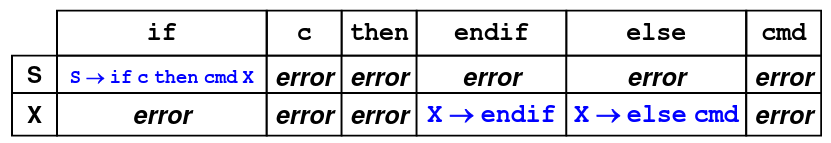
\includegraphics[width=0.8\textwidth]{/home/riccardoob/appunti/sistemi_operativi/images/16.png}
\end{figure}

\subsection{Sistemi fidati}

Il reference monitor impone le regole di sicurezza (Bell-La Padula) e ha le seguenti proprietà:

\paragraph{Mediazione completa} Le regole di sicurezza vengono applicate ad ogni accesso. Per motivi di efficienza, le soluzioni devono essere almeno parzialmente hardware.

\paragraph{Isolamento} il reference monitor e la base di dati sono protetti da modifiche non autorizzate.

\paragraph{Verificabilità} La correttezza del reference monitor deve essere provata, deve essere possibile dimostrare formalmente che il monitor impone le corrette regole di sicurezza e fornisce mediazione completa e isolamente.

Viene inoltre compilato un \textbf{audit file} dove vengono mantenuti gli eventi importanti per la sicurezza, come i tentativi di violazione alla sicurezza e le modifiche non autorizzate al nucleo di sicurezza.

















\chapter{Programmazione concorrente}

La programmazione concorrente è l'insieme delle tecniche, metodologie e strumenti per il supporto all'esecuzione di sistemi software da insieme di attività svolte simultaneamente.

Inizialmente implementata attraverso interruzioni (problemi con variabili comuni), oggi la programmazione concorrente è resa più facile dal reale parallelismo reso possibile da sistemi multiprocessore sempre più diffusi.

Le decisioni prese in merito di metodi di suddivisione dei processi e corretta sincronizzazione dipendono da tipo di applicazione e di architettura disponibile.

\section{Tipi di architettura}
\begin{figure}[H]
    \caption{Architettura single processor}
    \centering
    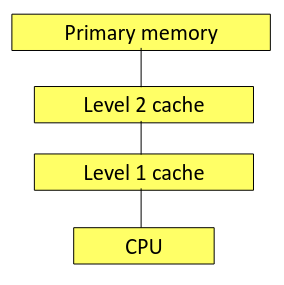
\includegraphics[width=0.45\textwidth]{/home/riccardoob/appunti/sistemi_operativi/images/10.png}
\end{figure}

\subsection{Sistemi multiprocessore}
\begin{figure}[H]
    \caption{Architettura memory multiprocessor}
    \centering
    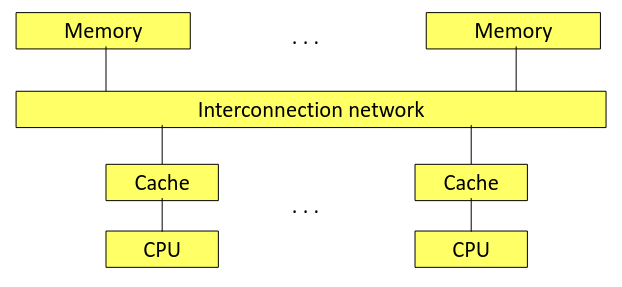
\includegraphics[width=0.6\textwidth]{/home/riccardoob/appunti/sistemi_operativi/images/11.png}
\end{figure}

Due modelli:
\begin{itemize}
    \item \textbf{UMA}: sistemi a multiprocessore con un numero ridotto di processori (da 2 a 30 circa)
    \begin{itemize}
        \item la rete di interconnessione realizzata tramite \textit{memory bus} o \textit{crossbar switch}
        \item Uniform Memory Access: tempo di accesso uniforme a da ogni processore a ogni locazione di memoria, chiamati anche \textbf{SMP} (symmetric multiprocessors).
    \end{itemize}
    \item \textbf{NUMA}: sistemi con un numero elevato di processori (decine o centinaia)
    \begin{itemize}
        \item memoria organizzata gerarchicamente per evitare congestioni sui bus
        \item rete di interconnessione composta da insieme di \textit{switches} e \textit{memorie} strutturato ad albero, distanze variabili dai processori
        \item Non Uniform Memory Access: tempo di accesso non uniforme
    \end{itemize}
\end{itemize}

\subsection{Distributed memory}
\begin{figure}[H]
    \caption{Architettura Multicomputers e Network systems}
    \centering
    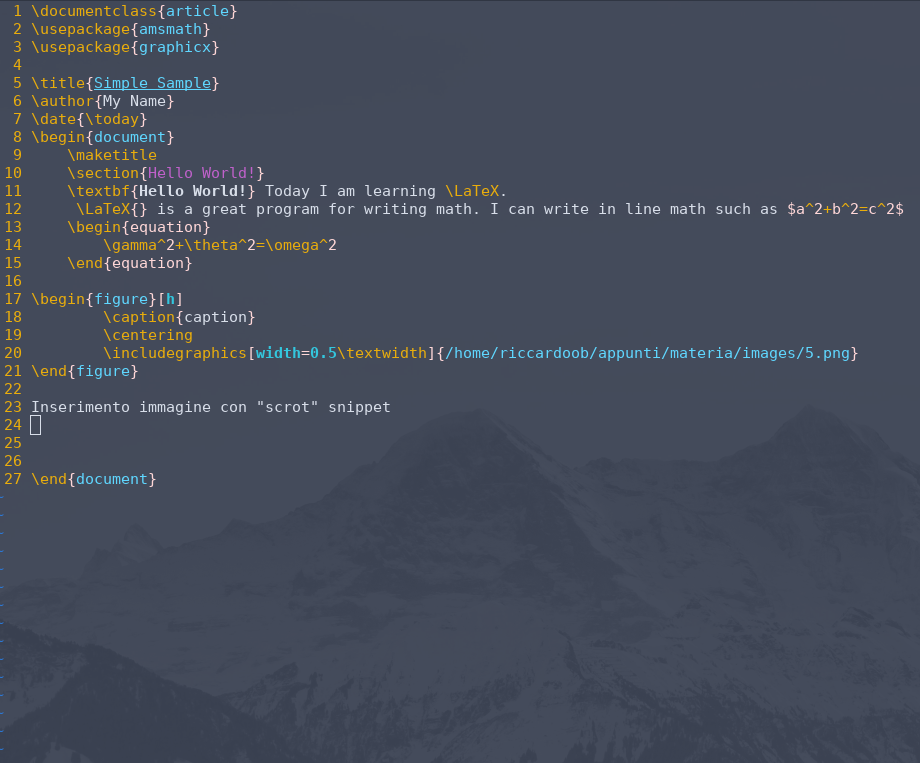
\includegraphics[width=0.6\textwidth]{/home/riccardoob/appunti/sistemi_operativi/images/12.png}
\end{figure}

Due modelli:
\begin{itemize}
    \item \textbf{Multcomputer}: processori e rete fisicamente vicini $\rightarrow$ \textit{tightly coupled machine}, la rete di interconnessione offre un cammine di comunicazione tra i processori ad alta velocità
    \item \textbf{Network systems}: nodi collegati da una rete locale o geografica $\rightarrow$ \textit{loosely coupled systems}.
\end{itemize}

I nodi di un distributed memory system possono essere o singoli processori o shared memory multiprocessor.

\subsection{Classificazione di Flynn}

La tassonomia di Flynn è basata su due concetti:
\begin{itemize}
    \item parallelismo a livello di istruzioni
    \begin{itemize}
        \item \textbf{single instruction stream}: esecuzione di un singolo flusso di istruzioni
        \item \textbf{multiple instruction stream}: esecuzione di più flussi in parallelo
    \end{itemize}
    \item parallelismo a livello di dati:
    \begin{itemize}
        \item \textbf{single data stream}: elaborazione di un singolo flusso sequenziale di dati
        \item \textbf{multiple data stream}: elaborazione di multipli flussi di dati paralleli
    \end{itemize}
\end{itemize}

\begin{figure}[H]
    \caption{Tassonomia di Flynn}
    \centering
    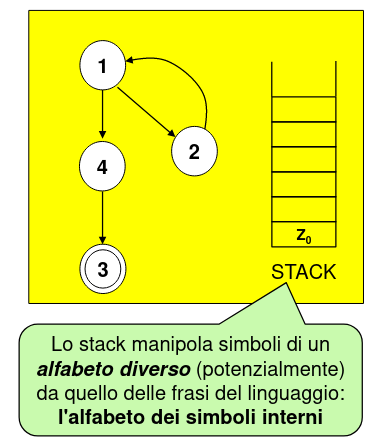
\includegraphics[width=0.7\textwidth]{/home/riccardoob/appunti/sistemi_operativi/images/13.png}
\end{figure}

\section{Applicazioni}

\begin{itemize}
    \item \underline{multithreaded} 
    \begin{itemize}
        \item strutturate come un insieme di processi per far fronte alla \textbf{complessità}, aumentare l'\textbf{efficienza} e per semplificare la programmazione.
        \item i processi possono condividere variabili
        \item esistono più processi che processori (generalmente)
        \item processi schedulati ed eseguiti indipendentemente
    \end{itemize}
    \item \underline{sistemi multitasking/distribuiti} 
    \begin{itemize}
        \item le coponenti dell'applicazione vengono eseguite su nodi collegati tramite opportuni mezzi di interconnessione
        \item comunicazione tramite scambio di messaggi
        \item tipicamente client server
    \end{itemize}
    \item \underline{applicazioni parallele} 
    \begin{itemize}
        \item risolvere un dato problema più velocemente sfruttando il parallelismo disponibile a livello HW
        \item a seconda del modello, istruzioni/thread/processi paralleli interagenti tra di loro
    \end{itemize}
\end{itemize}

\section{Processi non sequenziali e tipi di interazione}

\paragraph{Algoritmo} Procedimenti logico che deve essere eseguite per risolvere un determinato problema.

\paragraph{Programma} Descrizione di un algoritmo mediante un linguaggio, che rende possibile l'esecuzione da parte di un elaboratore.

\paragraph{Processo} Insieme ordinato degli eventi cui da luogo un operatore sotto il controllo di un programma.

\paragraph{Elaboratore} Entità astratta realizzata in hardware e parzialmente in software, in grado di eseguire programmi.

\paragraph{Evento} Esecuzione di una operazione, ogni evento determina una transizione di stato dell'elaboratore.

\subsection{Processo sequenziale}
Sequenza di stato attraverso i quali passa l'elaboratore durante l'esecuzione di un programma.

Un programma può evere più processi associati ad esso, ognuno di questi rappresenta l'esecuzione dello stesso codice con dati di ingresso (possibilmente) diversi.

Un processo può essere rappresentato tramite un grado orientato, detto \underline{grafo di precedenza} del processo, composto da nodi e archi orientati.
Ogni nodo rappresenta un evento corrispondente all'esecuzione di una operazione.

Il grafo di precedenza è a \textbf{ordinamento totale}, ovvero ogni nodo ha un predecessore e un successore.

\subsection{Processo non sequenziale}
Non sempre un processo possiede la proprietà dell'ordinamento totale, molti problemi possono essere risolti più naturalmente tramite processi non sequenziali.

Un \underline{processo non sequenziale} è una successione di eventi seconda una relazione d'ordine parziale.

L'esecuzione di un tale processo richiede un elaboratore in grado di supportare questo tipo di esecuzioni e un linguaggio di  programmazione adatto, non sequenziale.

\paragraph{Elaboratore non sequenziale}
\begin{itemize}
    \item sistemi multielaboratori (a)
    \item sistemi monoelaboratori (b)

\end{itemize}

\begin{figure}[H]
    \centering
    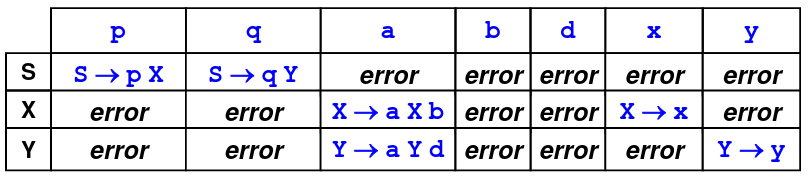
\includegraphics[width=0.8\textwidth]{/home/riccardoob/appunti/sistemi_operativi/images/17.png}
\end{figure}

\paragraph{Linguaggio non sequenziale} consente la descrizione di un insieme di attività concorrenti, sfruttando moduli che possono essere eseguiti in parallelo.

\underline{\textbf{Slide 32-63!!!!!!!!!!!!!!!!!!!!!!!!!!!!!!!!!!!!!!!!!!!!!!!!!!!!!!!!!!!!!!!!!!!!!!!!!!!!!!!!!!!!!!} } 

\section{Proprietà dei programmi}

\paragraph{Traccia dell'esecuzione} Sequenza degli stati attraversati dal sistema di elaborazione drante l'esecuzione del programma.

\paragraph{Stato} Insieme dei valori delle variabili definite nel programma e di quelle implicite.

\paragraph{Programmi sequenziali} Programmi che, su un insieme di dati D si ottiene sempre la stessa traccia.

\paragraph{Pogrammi concorrenti} L'esito dell'esecuzione dipende dalla sequenza cronologica di esecuzione delle istruzioni contenute, lo stesso insieme di dati D può dare una traccia diversa, \underline{non determinismo}.

Verificare che programmi di questo tipo siano corretti non è banale, un semplice debug non garantisce il soddisfacimento di una determinata proprietà.

\subsection{Proprietà dei programmi}

Una proprietà del programma P è un attributo che è sempre vero, data ogni traccia del programma P.

Le proprietà si possono classificare in due categorie:
\begin{itemize}
    \item \textbf{safety properties}
    \item \textbf{liveness properties}
\end{itemize}

\subsubsection{Safety}
É una proprietà che garantisce che durante l'esecuzione di P, non si entrerà \underline{mai} in uno stato "errato".

\subsubsection{Liveness}
É una proprietà che garantisce che durante l'esecuzione di P, \underline{prima o poi} si entrerà inuno stato "corretto".

Nel caso di programmi sequenziali, entrambe le proprietà devono essere realizzate, il programma deve restituire un risultato valido per ogni esecuzione e prima o poi terminare.

Per i programmi concorrenti, si aggiungono anche altri fattori alla completezza della safety e liveness:
\begin{itemize}
    \item Mutua esclusione nell'accesso a risorse (safety): nessun processo accede a una risorsa già occupata da un altro processo contemporaneamente
    \item Assenza di deadlock (safety): per ogni esecuzione non si devono verificare situazioni di blocco
    \item Assenza di starvation (liveness): prima o poi ogni processo potrà accedere akke risorse richieste
\end{itemize}


































































\chapter{Modello a memoria comune}

Esistono due modelli principale di interazione tra i processi:
\begin{itemize}
    \item memoria comune, ambiente globale con memoria condivisa
    \item scambio di messaggi, ambiente locale con memoria distribuita
\end{itemize}

In questo capitolo si analizza il modello a memoria comune.

Il sistema è visto come un insieme di \textbf{processi} e \textbf{oggetti}.

\begin{figure}[H]
    \centering
    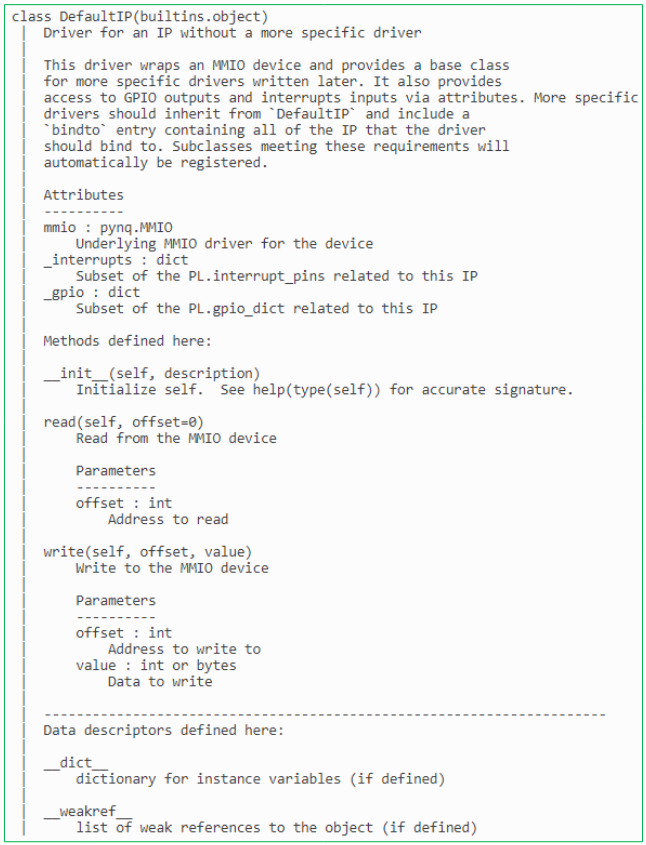
\includegraphics[width=0.5\textwidth]{/home/riccardoob/appunti/sistemi_operativi/images/18.png}
\end{figure}

In questo grafo, O1 e O4 sono risorse private, mentre O2 e O3 sono comuni.

Esistono due tipi di interazione tra processi:
\begin{itemize}
    \item \textbf{competizione}
    \item \textbf{cooperazione}
\end{itemize}

In questo modello, ogni applicazione viene strutturata come uninsieme di componenti, suddiviso in due sottoinsiemi disgiunti, i processi come componenti attivi e le risorse come componenti passivi.

\paragraph{Risorsa} Qualunque oggetto fisico di cui un processo necessita per portare a termine il suo compito.

Le risorse sono raggruppate in \underline{classi}, categorie che identificano l'insieme delle operazioni che un processo può eseguire.

\section{Gestore di una risorsa}

Per ogni risorsa R, il suo \textbf{gestore} definisce, in ogni istante $t$, l'insieme $SR(t)$ dei processi che hanno il diritto di operare su R.

Classificazione delle risorse in base alla condivisione:
\begin{itemize}
    \item \textbf{dedicata} se $SR(t)$ ha una cardinalità sempre $\le 1$
    \item \textbf{condivisa} in caso contrario
\end{itemize}

Classificazione delle risorse in base al tipo di allocazione:
\begin{itemize}
    \item \textbf{allocata staticamente} se $SR(t)$ è una costante $SR(t) = SR(t_0), \forall t$ 
    \item \textbf{allocata dinamicamente} se $SR(t)$ è una funzione del tempo
\end{itemize}
\begin{figure}[H]
    \caption{Tipologia di allocazione delle risorse}
    \centering
    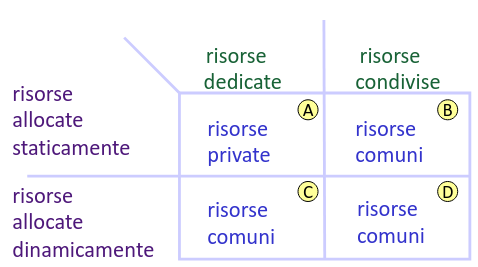
\includegraphics[width=0.65\textwidth]{/home/riccardoob/appunti/sistemi_operativi/images/19.png}
\end{figure}

Per ogni risorsa allocata \textit{staticamente}, l'insieme $SR(t)$ è definito prima che il programma inizi la propria esecuzione, il gestore della risorsa è il programmatore che stabilisce quale processo può operare su R.

Per ogni risorsa allocata \textit{dinamicamente}, il gestore $G_R$ definisce l'insieme $SR(t)$ in fase di esecuzione e quindi deve essere un componenete della stessa applicazione, nel quale l'allocazione viene decisa a run-time in base alle politiche date.

\subsection{Compiti del gestore di una risorsa}
Il gestore di una risorsa deve essere in grado di:
\begin{itemize}
    \item mantenere \textbf{aggiornato} l'insieme $SR(t)$ e lo stato di allocazione della risorsa
    \item fornire i \textbf{meccanismi} che un processo può utilizzare per ottenere i permessi per accedere alla risorsa e quindi entrare a far parte dell'insieme $SR(t)$ e per rilasciare questi permessi
    \item implementare la \textbf{strategia} di allocazione della risorsa e cioè definire quando, a chi e per quanto tempo allocare la risorsa
\end{itemize}

\subsection{Accesso a risorse}
Considerando un processo P che deve operare su una risorsa R di tipo T.

\subsubsection{Allocata staticamente}
Se R è allocata staticamente a P il processo, se appartiene a $SR(t)$ possiede il diritto di operae su R in qualunque istante.

\subsubsection{Allocata dinamicamente}
Se R è allocata dinamicamente a P, è necessario prevedere un gestore GR che implementa le funzioni di \underline{richiesta} e \underline{rilascio}, il processo deve richiedere accesso, eseguire operazione e rilasciare accesso.

\subsubsection{Allocata condivisa}
Se R è allocata come \textit{risorsa condivisa} è necessario assicurare che gli accessi avvengano in modo non divisibile: le funzioni di acecsso alla risorsa devono essere programmate come una classe di sezioni critiche utilizzando meccanismi di sincronizzazione).

\subsubsection{Allocata dedicata}
Se R è allocata come \textit{risorsa dedicata} essendo P l'unico processo che accede alla risorsa, non è necessario prevedere sincronizzazione.

\subsection{Specifica della sincronizzazione}

\paragraph{Regione critica condizionale [Hoare, Brinch-hansen]} Formalismo che consente di esprimere la specifica di qualunque \textbf{vincolo di sincronizzazione}.

\begin{minted}[bgcolor=lightgray,framesep=2mm,baselinestretch=1.2,fontsize=\footnotesize]{c}
region R << Sa; when(C) Sb;>>
\end{minted}

Il corpo della region rappresenta una operazione da eseguire sulla risorsa condivisa R, è la \textbf{sezione critica} che deve essere eseguita in mutua esclusione con le altre operazioni.

Vengono eseguite le istruzioni \texttt{Sa} e, non appena C è vera, \texttt{Sb}.

\begin{figure}[H]
    \centering
    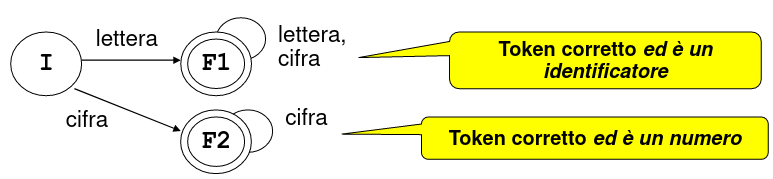
\includegraphics[width=0.5\textwidth]{/home/riccardoob/appunti/sistemi_operativi/images/20.png}
\end{figure}

\subsection{Casi particolari}
\begin{itemize}
    \item \texttt{region R << S; >>} mutua esclusione senza ulteriori vincoli
    \item \texttt{region R << when(C) >>} specifica di un vincolo di sincronizzazione: P deve attendere che C si verifichi
    \item \texttt{region R << when(C) S; >>} in questo caso C è una precondizione necessaria per eseguire S
\end{itemize}

\section{Il problema della mutua esclusione}
Il problema della mutua esclusione nasce quando più processi possono avere accesso a variabili comuni, la regola impone che le operazioni non si sovrappongano nel tempo, nessun vincolo è imposto sull'ordine delle operazioni.

\paragraph{Sezione critica}
Una sequenza di istruzioni che accede e modifica un insieme di variabili comuni prende il nome di sezione critica.

La regola di mutua esclusione stabilisce che sezioni critiche della stessa classe non pososno essere in esecuzione contemporaneamente.

Il protocollo di esecuzione di una sezione critica è il seguente:
\begin{minted}[bgcolor=lightgray,framesep=2mm,baselinestretch=1.2,fontsize=\footnotesize]{c}
<prologo>
S;
<epilogo>
\end{minted}

Nel prologo si richiede e ottiene l'autorizzazione a eseguire la sezione, nell'epilogo si rilascia la risorsa.

\section{Strumenti linguistici per la programmazione di interazioni}

\subsection{Semaforo}
É uno strumento di basso livello, realizzato dal kernel della macchina, utile a risolvere qualsiasi problema di sincronizzazione.

L'eventuale attesa nell'esecuzione può essere realizzata utilizzando i meccanismi di gestione dei thread (sospensione, riattivazione) offerti dal kernel.

Un semaforo è una variabile \textit{interna non negativa} alla quale è possibile accedere solo tramite le due operazioni \texttt{P} e \texttt{V}.

Specifica delle operazioni di un semaforo:
\begin{minted}[bgcolor=lightgray,framesep=2mm,baselinestretch=1.2,fontsize=\footnotesize]{c}
void P(semaphore s):
    region s << when(val>0) val--; >>


void V(semaphore s):
    region s << val++; >>
\end{minted}

Dato un semaforo S, siano:
\begin{itemize}
    \item $\texttt{val}_\texttt{s}$: valore dell'intero non negativo associato al semaforo
    \item $\texttt{I}_\texttt{s}$: valore interno maggiore di zero di inizializzazione
    \item $\texttt{nv}_\texttt{s}$: numero di volte che l'operazione \texttt{V(s)} è stata eseguita
    \item $\texttt{np}_\texttt{s}$: numero di volte che l'operazione \texttt{P(s)} è stata eseguita
\end{itemize}

\subsubsection{Relazione di invarianza}
Ad ogni istante possiamo esprimere il valore del semaforo come $\texttt{val}_\texttt{s} = \texttt{I}_\texttt{s} + \texttt{nv}_\texttt{s} - \texttt{np}_\texttt{s}$ da cui si ottiene $\texttt{np}_\texttt{s}\le \texttt{I}_\texttt{s}+\texttt{nv}_\texttt{s}$

La relazione di invarianza è sempre soddisfatta (safety property), si può usare questa proprietà per dimostrare formalmente le proprietà dei programmi concorrenti.

\subsubsection{Utilizzo}
Il semaforo è uno strumento generale che consente la risoluzione di qualunque problema di sincronizzazione, ne esistono però specializzazioni utili in particolari casi:
\begin{itemize}
    \item semafori mutua esclusione
    \item semafori evento
    \item semafori binari composti
    \item semafori condizione
    \item semafori risorsa
    \item semafori privati
\end{itemize}

\subsubsection{Semaforo mutua esclusione}

Viene inizializzato a 1 ed è usato per realizzare le sezioni critiche di una stessa classe.
\begin{minted}[bgcolor=lightgray,framesep=2mm,baselinestretch=1.2,fontsize=\footnotesize]{java}
class risorsa {
    semaphore mutex = 1;
    public void op1() {
        P(mutex);
        <sez. critica>
        V(mutex);
    }
}
\end{minted}

Le seguenti condizioni sono soddisfatte:
\begin{itemize}
    \item sezione critiche della stessa classe devono essere eseguite in modo mutualmente esclusivo
    \item non deve essere possibile il verificarsi di deadlock
    \item un processo fuori dalla sezione critica non deve bloccare l'entrata ad altri processi
\end{itemize}

\subsection{Mutua esclusione tra gruppi e processi}
In alcuni casi può essere utile consentire a più processi di eseguire contemporaneamente la stessa operazione su una risorsa, ma non operazioni diverse.

Data la risorsa condivisa \texttt{ris} e indicate con $\texttt{op}_\texttt{1} \dots \texttt{op}_\texttt{n}$ le n operazioni eseguibili su \texttt{ris}, si vuole garantire che i processi possano eseguire contemporaneamente $\texttt{op}_\texttt{i}$.

Lo schema è il solito prologo, operazione, epilogo:
\begin{itemize}
    \item il \underline{prologo} deve sospendere il processo che ha chiamato l'operazione se sulla risorsa sono in esecuzione operazioni diverse, altrimenti deve procedere
    \item l'\underline{epilogo} deve liberare la mutua esclusione solo se il processo che lo esegue è l'unico processo in esecuzione sulla risorsa
\end{itemize}

Si definisce una \textit{semaforo mutex} per la mutua esclusione tra operazioni e un'altro per le sezioni critiche prologo e epilogo.

\begin{minted}[bgcolor=lightgray,framesep=2mm,baselinestretch=1.2,fontsize=\footnotesize]{java}
semaphore mutex=1, m_i=1;

public void op_i() {
    P(m_i);
    cont_i++;
    if (cont_i==1) P(mutex);
    V(m_i);
    <corpo operazione>
    P(m_i);
    cont_i--;
    if (cont_i==0) V(mutex);
    V(m_i);
}
\end{minted}

Questo schema è applicabile alla casistica di lettura scrittura su file: più processi possono leggere un file contemporaneamente mentre una sola può modificare.

\subsection{Semafori evento - scambio di messaggi temporali}
Un semaforo \textbf{evento} è un semaforo binario utilizzato per imporre un vincolo di precedenza tra operazioni e processi.

\subsubsection{Esempio}
$\texttt{op}_a$ deve essere eseguita da $\texttt{P}_1$ solo dopo che $\texttt{P}_2$ ha eseguito $\texttt{op}_b$.

Si introduce un semaforo \texttt{sem} inizializzato a zero:
\begin{itemize}
    \item prima di eseguire $\texttt{op}_a$, $\texttt{P}_1$ esegue \texttt{P(sem)}
    \item dopo aver eseguite $\texttt{op}_b$, $\texttt{P}_2$ esegue \texttt{V(sem)}
\end{itemize}

\begin{figure}[H]
    \centering
    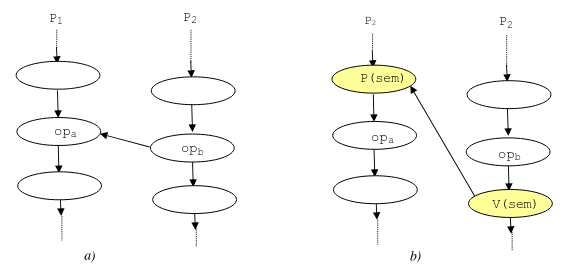
\includegraphics[width=0.6\textwidth]{/home/riccardoob/appunti/sistemi_operativi/images/21.png}
\end{figure}

\subsubsection{Problema del rendez-vous}
Due processi \texttt{P}$_1$ e \texttt{P}$_2$ eseguono ciascuno due operazioni, \texttt{p}$_a$ e \texttt{p}$_b$ il primo e \texttt{q}$_a$ e \texttt{q}$_b$ il secondo.

\begin{mdframed}[topline=false,bottomline=false,rightline=false]
    \textbf{Vincolo di rendez-vous}\\
    L'esecuzione di \texttt{p}$_b$ da parte di \texttt{P}$_1$ e \texttt{q}$_b$ da parte di \texttt{P}$_2$ possno inziare solo dopo che entrambi i processi hanno completato la loro prima operazione( \texttt{p}$_a$ e \texttt{q}$_a$).
\end{mdframed}

Ogni processo segnala quando arriva al punto di incontro e attende, si utilizzano due semafori \texttt{sem1} e \texttt{sem2}.

\begin{figure}[H]
    \centering
    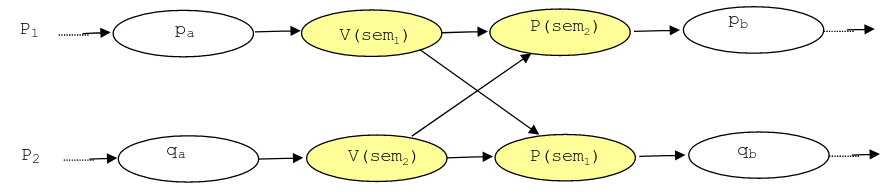
\includegraphics[width=0.6\textwidth]{/home/riccardoob/appunti/sistemi_operativi/images/22.png}
\end{figure}

Si può generalizzare il concetto del rendez-vous a \texttt{N} processi, introducendo il concetto di barriera di sincronizzazione.

\subsubsection{Barriera di sincronizzazione}
L'esecuzione di ogni operazione \texttt{P}$_{ib}$ è subordinata al completamento di tutte le istruzioni \texttt{P}$_{ia} (i=1,\dots,N)$

\begin{figure}[H]
    \centering
    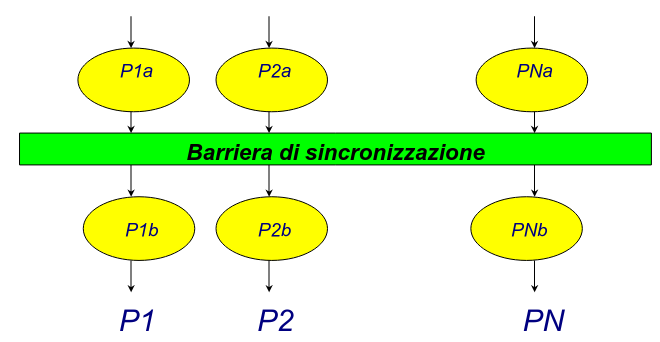
\includegraphics[width=0.6\textwidth]{/home/riccardoob/appunti/sistemi_operativi/images/23.png}
\end{figure}

\begin{minted}[bgcolor=lightgray,framesep=2mm,baselinestretch=1.2,fontsize=\footnotesize]{java}
// condivise
semaphore mutex = 1;
semaphore barriera = 0;
int completati = 0;
//struttura thread i-esimo P_i
p(mutex);
completati++;
if (completati==N)
    v(barriera);
v(mutex);
p(barriera);
v(barriera);
\end{minted}

\subsection{Semafori binari composti - scambio di dati}
Due processi \texttt{P}$_1$ e \texttt{P}$_2$ si scambiano dati di tipo \texttt{T} utilizzando una memoria condivisa.

Gli accessi al buffer devono essere mutuamente esclusivi, \texttt{P}$_2$ può \textit{prelevare} un dato solo dopo che \texttt{P}$_1$ lo ha \textit{inserito}, \texttt{P}$_1$, \textit{prima} di inserire un dato, deve attendere che \texttt{P}$_2$ abbia \textit{estratto} il precedente.

\begin{figure}[H]
    \centering
    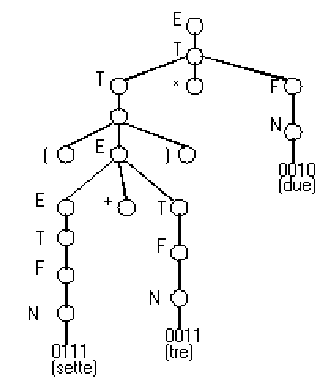
\includegraphics[width=0.6\textwidth]{/home/riccardoob/appunti/sistemi_operativi/images/24.png}
\end{figure}

Per implementare questa funzionalità si utilizzano due semafori:
\begin{itemize}
    \item \texttt{vu}, per realizzare l'attesa di \texttt{P}$_1$ in caso di buffer pieno
    \item \texttt{pn}, per realizzare l'attesa di \texttt{P}$_2$ in caso di buffer vuoto
\end{itemize}

\begin{multicols}{2}
    \begin{minted}[bgcolor=lightgray,framesep=2mm,baselinestretch=1.2,fontsize=\footnotesize]{java}
void invio(T dato) {
    P(vu);
    inserisci(dato);
    V(pn);
}


//P1
while (true) {
    //prepara messaggio
    invio(msg);
}
    \end{minted}
    \columnbreak
    \begin{minted}[bgcolor=lightgray,framesep=2mm,baselinestretch=1.2,fontsize=\footnotesize]{java}
T ricezione() {
    T dato;
    P(pn);
    dato = estrai();
    V(vu);
    return dato;
}
//P2
while (true) {
    M = ricezione();
    //consuma
}
    \end{minted}
\end{multicols}

\begin{mdframed}[topline=false,bottomline=false,rightline=false]
    Un semaforo binario composto è un insieme di semafori usato in modo tale che:
    \begin{itemize}
        \item uno solo di essi sia inizializzato a 1 e tutti gli altri a 0
        \item ogni processo che usa questi semafori esegue sempre sequenze che iniziano con la P su uno di questi e termina con la V su un altro
    \end{itemize}
\end{mdframed}
\subsection{Semafori condizione}
In alcuni casi, l'esecuzione di una istruzione \texttt{S}$_1$ su una risorsa \texttt{R} è subordinata a una condizione \texttt{C} 
\begin{minted}[bgcolor=lightgray,framesep=2mm,baselinestretch=1.2,fontsize=\footnotesize]{C}
void op1(): region R << when(C) S1; >>
\end{minted}
\begin{itemize}
    \item \texttt{op1()} è una regione critica
    \item \texttt{S1} ha come precondizione la validità della condizione logica \texttt{C}
\end{itemize}

Il processo deve sospendersi se la condizione non si verifica, e deve uscire dalla regione per permettere ad altri processi di eseguire operazioni su \texttt{R} per rendere vera la condizione \texttt{C}.

\begin{figure}[H]
    \centering
    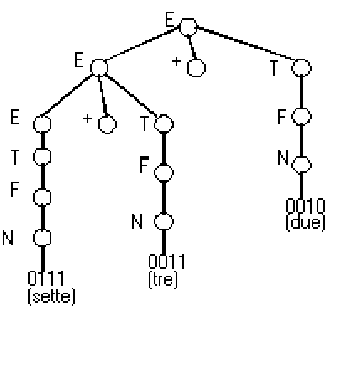
\includegraphics[width=0.7\textwidth]{/home/riccardoob/appunti/sistemi_operativi/images/25.png}
\end{figure}

Lo schema \texttt{(a)} presuppone una forma di attesa attiva da parte del processo che non trova soddisfatta la condizione.

Nello schema \texttt{(b)} si realizza la region \textbf{sospendendo} il processo sul semaforo \texttt{sem} da associare alla condizione, si rende necessaria un'altra operazione \texttt{op2} che abbia \texttt{C} come postcondizione e che chiami nel suo contesto \texttt{V(sem)}.

\vspace{-0.5cm}
\subsubsection{Schema attesa circolare}
\vspace{-0.5cm}
\begin{multicols}{2}
    \begin{minted}[bgcolor=lightgray,framesep=2mm,baselinestretch=1.2,fontsize=\footnotesize]{java}
public void op1() {
    P(mutex);
    while (!C) {
        csem++;
        V(mutex);
        P(sem);
        P(mutex);
    }
    S1;
    V(mutex);
}
    \end{minted}
    \columnbreak
    \begin{minted}[bgcolor=lightgray,framesep=2mm,baselinestretch=1.2,fontsize=\footnotesize]{c}
public void op2() {
    P(mutex);
    if (csem > 0) {
        csem--;
        V(sem);
    }
    V(mutex);
}
    \end{minted}
\end{multicols}

\subsubsection{Schema passaggio testimone}

\begin{multicols}{2}
    \begin{minted}[bgcolor=lightgray,framesep=2mm,baselinestretch=1.2,fontsize=\footnotesize]{java}
public void op1() {
    P(mutex);
    if (!C) {
        csem++;
        V(mutex);
        P(sem);
        csem--;
    }
    S1;
    V(mutex);
}
    \end{minted}
    \columnbreak
    \begin{minted}[bgcolor=lightgray,framesep=2mm,baselinestretch=1.2,fontsize=\footnotesize]{java}
public void op2() {
    P(mutex);
    S2;
    if (C && csem > 0)
        V(sem);
    else
        V(mutex);
}
    \end{minted}
\end{multicols}

Il metodo del testimone è il più efficiente, tuttavia è possibile risvegliare \textit{un solo} processo alla volta e la condizione \texttt{C} non può dipendere da parametri locali a \texttt{op1()}.

\subsubsection{Gestione di un pool di risorse equivalenti}

Si consideri un \textbf{pool} di \texttt{N} risorse tutte uguali, ciascun processo può operare su una qualsiasi risorsa del pool, purché \textit{libera}.

É necessario un \textbf{gestore} che mantenga aggiornato lo stato delle risorse:
\begin{itemize}
    \item ogni processo, prima di operare su una risorsa \textit{chiede al gestore} l'allocazione di una di esse
    \item il gestore \textbf{assegna} al processo una risorsa libera, passandogli l'\textbf{indice} relativo
    \item il processo opera sulla risorsa
    \item al termine il processo \textbf{rilascia} la risorsa a gestore
\end{itemize}

\begin{minted}[bgcolor=lightgray,framesep=2mm,baselinestretch=1.2,fontsize=\footnotesize]{java}
class Gestore {
    semaphore mutex = 1;
    semaphore sem = 0;
    int csem = 0;
    boolean libera[N];
    int disponibili = N;
    {for (int i = 0; i < N; i++) libera[i]=true;}
    
    public int richiesta() {
        int i = 0;
        P(mutex);
        if (disponibili == 0) {
            csem++;
            V(mutex);
            P(sem);
            csem--;
        }
        while (!libero[i]) i++;
        libero[i] = false;
        V(mutex);
        return i;
    }

    public void rilascio(int r) {
        P(mutex);
        libero[r] = true;
        disponibili++;
        if (csem > 0) 
            V(sem);
        else 
            V(mutex);
    }
}
\end{minted}

Schema di esempio di un generico processo che vuole accedere a una risorsa \texttt{ris}.

\begin{minted}[bgcolor=lightgray,framesep=2mm,baselinestretch=1.2,fontsize=\footnotesize]{java}
process P {
    int ris;
    ...
    ris = G.richiesta();
    //<utilizzo risorsa>
    G.rilascio();
    ...
}
\end{minted}

\subsection{Semaforo risorsa}
I semafori risorsa sono semafori generali, ovvero possono assumere qualunque valore maggiore di zero.

Sono utilizzato per realizzare allocazione per risorse equivalenti, il valore del semaforo rappresenta il \textbf{numero di risorse libere}.

\subsubsection{Gestione di un pool di risorse equivalenti}
Si può utilizzare un semaforo risorsa per gestire un pool di risorse, si crea un unico semaforo \texttt{n\_ris} inizializzato con un valore uguale al numero di risorse, si eseguono P(n\_ris) in allocazione e V(n\_ris) in rilascio.

\begin{minted}[bgcolor=lightgray,framesep=2mm,baselinestretch=1.2,fontsize=\footnotesize]{java}
class Gestore {
    semaphore mutex = 1;
    semaphore n_ris = N;
    boolean libero[N];

    {for (int i = 0; i < N; i++)
        libera[i] = true;}

    public int richiesta() {
        int i = 0;
        P(n_ris);
        P(mutex);
        while (!libero[i]) i++;
        libero[i] = false;
        V(mutex);
        return i;
    }
    
    public void rilascio (int r) {
        P(mutex);
        libero[r] = true;
        V(mutex);
        V(n_ris);
    }

}
\end{minted}

\subsubsection{Problema dei produttori/consumatori}
Si crea un buffer di \texttt{n} elementi, strutturato come una coda
\begin{minted}[bgcolor=lightgray,framesep=2mm,baselinestretch=1.2,fontsize=\footnotesize]{java}
coda_di_n_T buffer;
semaphore pn = 0;
semaphore vu = 0;
semaphore mutex = 1;
\end{minted}

\begin{multicols}{2}
    \begin{minted}[bgcolor=lightgray,framesep=2mm,baselinestretch=1.2,fontsize=\footnotesize]{java}
void invio(T dato) {
    P(vu);
    P(mutex);
    buffer.inserisci(dato);
    V(mutex);
    V(pn);
}
    \end{minted}
    \columnbreak
    \begin{minted}[bgcolor=lightgray,framesep=2mm,baselinestretch=1.2,fontsize=\footnotesize]{java}
void ricezione() {
    T dato;
    P(pn);
    P(mutex);
    dato = buffer.estrai();
    V(mutex);
    V(vu);
    return dato;
}
    \end{minted}
\end{multicols}

\subsection{Semafori privati - specifiche strategie di allocazione}
Qualora si voglia realizzare una politica di gestione delle risorse particolare, la decisione se permettere o no l'esecuzione a un dato processo dipende dal verificarsi duna specifica \textbf{condizione di sincronizzazione}.

Queste condizioni vengono espresse in termini di variabili che rappresentano lo \textbf{stato della risorsa} e variabili \textit{locali} ai singoli processi.

Sorge il problema di quale processo mettere in esecuzione, risolvibile definendo una \textbf{politica di risveglio} dei processi bloccati.

Nei casi precedenti la politica di risveglio era dipendente dalla specifica implementazione dell'algoritmo all'interno della V, solitamente realizzato con risveglio FIFO.

\begin{mdframed}[topline=false,bottomline=false,rightline=false]
    Un semaforo \texttt{s} si dice \textbf{privato} per un processo quando solo tale processo può eseguire la primitiva \texttt{P} su semaforo \texttt{s}. La primitiva \texttt{V} può essere eseguita da qualunque processo.
\end{mdframed}

Un semaforo privato viene inizializzato con valore \textbf{zero}.

Il processo che acquisisce la risorsa può sospendersi sul suo semaforo privato se la condizione di sincronizzazione non è soddisfatta, chi rilascia tale risorsa, può risvegliare uno dei processi sospesi (in base alla politica definita) mediante una \texttt{V} sul semaforo privato del processo scelto.

Schema generale:

\begin{minted}[bgcolor=lightgray,framesep=2mm,baselinestretch=1.2,fontsize=\footnotesize,escapeinside=||,mathescape=true]{java}
class Gestore {
    <struttura dati gestore>;
    semaphore mutex = 1;
    semaphore priv[n] = {0, 0, |$\dots$|, 0} //semafori privati

    public void acquisizione (int i) {
        P(mutex);
        if (<condizione di sincronizzazione>) {
            <allocazione della risorsa>;
            V(priv[i]);
        }
        else {
            <registrare la sospensione del processo>;
        }
        V(mutex);
        P(priv[i]);
    }

    public void rilascio() {
        int i;
        P(mutex);
        <rilascio risorsa>;
        if (<min 1 processo soddisfa sync condition>) {
            <scelta tra sospesi del Pi da riattivare>;
            <allocazione risorsa a Pi>;
            <registrare Pi come non sospeso>;
            V(priv[i]);
        }
        V(mutex);
    }
}
\end{minted}

La sospensione del processo in acqusizione, se la condizione di sincronizzazione non è soddisfatta, deve avvenire \textit{al di fuori dell sezione critica}, altrimenti si impedirebbe a un processo che rilascia la risorsa di accedere a sua volta alla sezione critica.

La soluzione mostrata può presentare inconvenienti:
\begin{itemize}
    \item la \texttt{P} sul privato viene \textbf{sempre eseguita}, anche se non necessario
    \item il codice dell'assegnazione della risorsa è \textit{duplicato} nelle due procedure
\end{itemize}

Correggendo questi problemi:

\begin{minted}[bgcolor=lightgray,framesep=2mm,baselinestretch=1.2,fontsize=\footnotesize]{java}
class Gestore() {
    <struttura dati gestore>;
    semaphore mutex = 1;
    semaphore priv[n] = {0, 0, |$\dots$|, 0}; //semafori privati

    public void acqusizione(int i) {
        P(mutex);
        if (! <condizione di sincronizzazione) {
            <registrare sospensione processo>;
            V(mutex);
            P(priv[i]);
            <registrare processo come non sospeso>;
        }
        <allocazione risorsa>;
        V(mutex);
    }

    public void rilascio() {
        int i;
        P(mutex);
        <rilascio risorsa>;
        if (<min 1 processo soddisfa sync condition>) {
            <scelta tra sospesi del Pi da riattivare>;
            V(priv[i]);
        }
        else
            V(mutex);
    }
}
\end{minted}

Il risveglio segue lo schema del \textbf{passaggio del testimone}.

A differenza della soluzione precedente è più complesso realizzare la riattivazione di più processi che hanno condizione di sincronizzazione verificata: il processo che rilascia la risorsa attiva al massimo un processo, il quale dovrà a sua volta provvedere a riattivare eventuali processi.

\subsubsection{Esempio 1}
Su un buffer di N celle di memoria, più produttori possono depositare messaggio di dimensione diversa.

\textbf{Politica di gestione}: tra più produttori ha priorità di accesso quello che fornisce il messaggio di dimensione maggiore.

\textbf{Condizione di sincronizzazione}: il deposito può avvenire se c'è abbastanza spazio per memorizzare il messaggio e non ci sono produttori in attesa.

Il \textbf{prelievo} di messaggi da parte di un consumatore riattiva il produttore con messaggio con \textbf{dimensione maggiore} (se spazio sufficiente nel buffer), se lo \textit{spazio non è sufficiente}, nessun produttore viene riattivato.

Soluzione:
\begin{minted}[bgcolor=lightgray,framesep=2mm,baselinestretch=1.2,fontsize=\footnotesize,escapeinside=||,mathescape=true]{java}
class Buffer {
    int richiesta[num_proc] = 0; //numero di celle richieste da Pi
    int sospesi = 0;
    int vuote = n; //numero celle vuote del buffer

    semaphore mutex = 1;
    semaphore priv[num_proc] = {0, 0, |$\dots$|, 0};

    public void acqusizione(int m, int i) {
        // m dim mess, i id processo
        P(mutex);
        if (sospesi == 0 && vuote >= m) {//assegna m celle a Pi
            vuote = vuote - m;
            V(priv[i]);
        }
        else {
            sospesi++;
            richiesta[i] = m;
        }
        V(mutex);
        P(priv[i]);
    }
    
    public void rilascio(int m) {
        int k;
        P(mutex);
        vuote += m;
        while (sospesi != 0) {
            <individuazione del Pk con max richiesta>;
            if (richiesta[k] <= vuote) { //assegno a Pk
                vuote = vuote - richiesta[k];
                richiesta[k] = 0;
                sospesi--;
                V(priva[k]);
            }
            else {
                break;
            }
        }
        V(mutex);
    }
}
\end{minted}

\subsubsection{Esempio 2}
Un insieme di processi utilizza un insieme di risorse comuni R1, R2, \dots, Rn. Ogni processo può utilizzare una qualunque delle risorse.

\textbf{Politica di gestione}: a ogni processo è assegnata una \textbf{priorità}, in fase di riattivazione dei processi sospesi, viene scelto quello con la \textit{massima priorità}.

\textbf{Condizione sincronizzazione}: accesso consentito solo se esiste una \textit{risorsa libera}.











































































\end{document}
